\section{Программная реализация}
В данной главе рассмотрены уже существующие решения, связанные с генерацией отчетов, 
а также детально описана программная реализация полученной в рамках настоящей работы системы.

\subsection{Обзор существующих решений для генерации отчетов}
На данный момент существует множество систем, которые могут использоваться
для автоматической генерации отчетов по уже имеющимся данным: 
среди них есть, как простые, которые предоставляют интерфейс для построения
простых табличных отчетов на основе массива данных (например BandedReportGenerator\cite{BandedReportGenerator}),
так и более комплексные, предоставляющие возможность составления отчетов на основе 
языка RDL (Report Definition Language\cite{rdl_spec}), генерировать OLAP-кубы\cite{olap},
самостоятельно работать с подключением к источнику данных и т.д.

В рамках данного раздела рассмотрены два наиболее популярных программных комплекса
для работы с отчетами: ``SAP Crystal Reports''\cite{crystal_reports} и 
``SQL Server Reporting Services''\cite{sql_reporting} для Microsoft SQL Server, 
оценены их достоинства и недостатки, а также обосновано решение, принятое к реализации.

\subsubsection{SAP Crystal Reports}
\begin{figure}[!ht]
\begin{center}
\hspace*{-1cm} 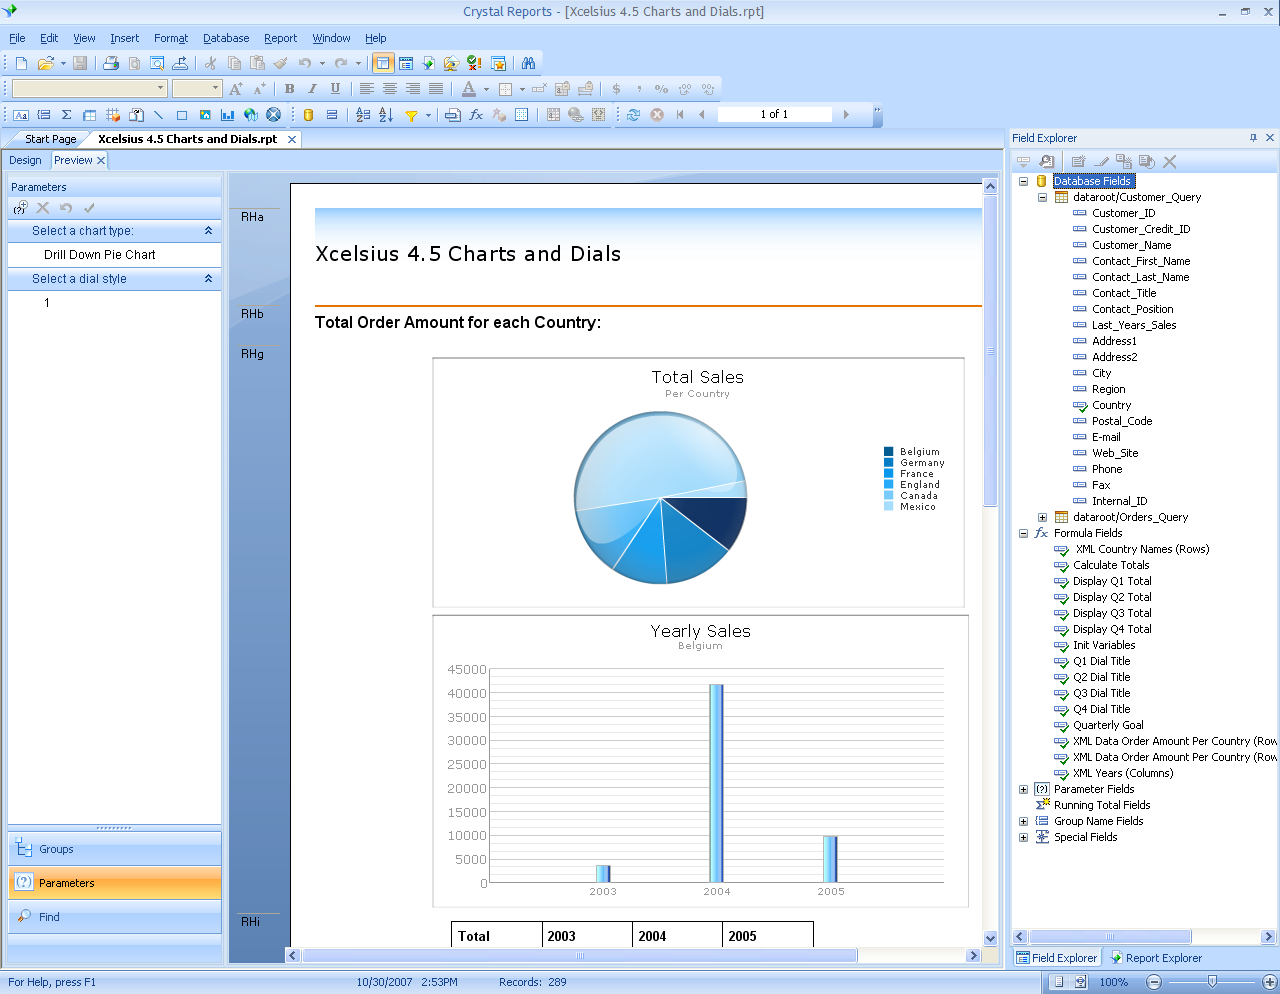
\includegraphics[scale=0.4]{../resources/CrystalReports2008.png}
\caption{Скриншот Crystal Reports 2008}
\label{gr:crystal_screenshot}
\end{center}
\end{figure}

\textit{Crystal Reports} является наиболее популярным продуктом компании SAP, состоит из
множества приложений таких как ``Crystal Reports Server'', ``Crystal Reports Viewer'',
``Crystal Reports Designer'', а так же плагина для Microsoft Visual Studio, позволяющего
составлять шаблоны отчетов в среде разработки.
 
\paragraph{Достоинства}
\begin{itemize}
\item{
Простой интерфейс для построения несложных отчетов.
}
\item{
Возможность генерации OLAP-кубов\cite{olap}, удобное представление
древообразной структуры отчета, описанной в \ref{section:stat_reports_task}.
}
\item{
Реализована работа с базой данных.
}
\item{
Реализована возможность графической интерпретации отчетов.
}
\end{itemize}

\paragraph{Недостатки}
\begin{itemize}
\item{
Отсутствие готовых решений для генерации отчетов через веб-интерфейс.
}
\item{
Недостаточная гибкость вычисления показателей, ограниченная пользовательскими формулами.
}
\item{
Инкапсуляция методов обработки данных, ограничивающая возможность оптимизировать
запросы к СУБД.
}
\end{itemize}

\subsubsection{SQL Server Reporting Services}
\begin{figure}[!ht]
\begin{center}
\hspace*{-1cm} 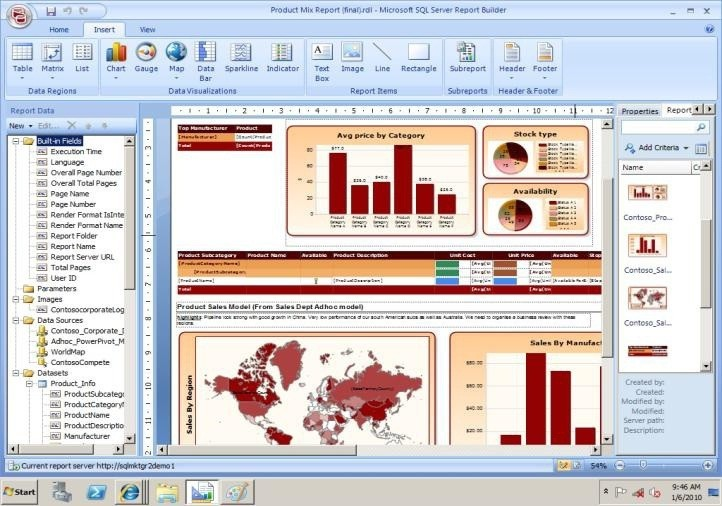
\includegraphics[scale=0.7]{../resources/SQLReporting.jpg}
\caption{Скриншот приложения Microsoft SQL Server Reporting Services 2008}
\label{gr:crystal_screenshot}
\end{center}
\end{figure}
Комплекс приложений \textit{SQL Server Reporting Services} создавался как конкурент для
\textit{SAP Crystal Reports}. В нем реализованы по сути те же базовые инструменты для конструирования
и просмотра отчетов, но при этом добавлены некоторые элементы функциональности, 
позволяющие Reporing Services занимать достойную позицию на рынке Business Intellegence технологий.

\paragraph{Достоинства}
\begin{itemize}
\item{
Более тесная интеграция с СУБД Microsoft SQL Server, которая в соответствии 
с нефункциональными требованиями к системе (см. \ref{part:requirements}) должна быть
использована в качестве хранилища данных.
}
\item{
Реализованы модули просмотра отчетов для ASP.NET\cite{sql_reporting}, что позволяет
реализовать генератор в виде веб-приложения.
}
\item{
Язык RDL\cite{rdl_spec}, реализованный на основе XML, позволяет специфицировать вид шаблона отчета,
на основе которого может быть сгенерирован отчет для пользователя, как через 
веб-интерфейс, так и с использованием Desktop-приложения.
}
\end{itemize}

\paragraph{Недостатки} В SQL Reporting Services присутствуют те же недостатки, что и в случае
с Crystal Reports, за исключением возможности генерации отчетов через веб-интерфейс.

\subsubsection{Результаты обзора}
Оба рассмотренные в предыдущих разделах программных продукта 
обладают неоспоримыми достоинствами, предлагая, как конечному пользователю, так и разработчику,
большой диапазон инструментов, позволяющих решать самый широкий круг задач.
Однако на первом этапе реализации системы было принято решение избежать их использования
в связи с серьезными рисками, возникающими в случае их применения в связи с
высокой степенью инкапсуляции механизмов построения отчетов в этих системах.

Возможные проблемы, вызванные инкапсуляцией включают:
\begin{itemize}
\item{
Невозможность достаточно тонкой настройки генератора может привести к несоответствиям в результате
работы генератора отчетов и требований к ним.
}
\item{
Невозможность оптимизации запросов к СУБД. Это может привести к тому, что при большом количестве данных
время генерации отчетов будет выходить за рамки, оговоренные в требованиях.
}
\end{itemize}

Таким образом в рамках данной работы было необходимо разработать оригинальный 
алгоритм генерации отчетов, результат работы которого должен удовлетворять требованиям,
описанным в первой главе.

При этом, учитывая факт использования в системе Microsoft SQL Server, не стоит исключать
возможность генерации более простых отчетов с помощью SQL Reporting Services, которое
пользователь сможеть осуществить самостоятельно при наличии доступа к серверу СУБД.

\subsection{Архитектура приложения}


\subsubsection{Фреймворк Yii}
Для программной реализации приложения был выбран фреймворк Yii\cite{yii}, написанный на языке
программирования PHP. Он реализован в соответствии с паттерном проектирования MVC\cite{gamma},
предполагая разделение на различные компоненты следующих частей приложения:
\begin{itemize}
\item{
Части, составляющие модель данных
}
\item{
Части, отвечающие за взаимодействиее системы и пользователя
}
\item{ 
Часть, связанная с пользовательским интерфейсом
}
\end{itemize}

Yii унаследовал многие достоинства других фреймворков для PHP, таких как Symfony или Zend, 
при этом обладая многими преимуществами по сравнению с ними, такими как высокая производительность,
удачные архитектурные решения для использования Ajax в совокупности с jQuery и т.д.

\paragraph{Жизненный цикл запроса}
Yii реализует сразу оба типичных решения при обработке HTTP-запросов пользоваеля, описанные в \cite{fowler}:
FrontContoller (на рис. \ref{gr:yiirequestflow} YiiApp) получает данные запроса, затем на основе
адреса запроса и конфигурации маршрутов выбирает подходящий PageController и action, который формирует текст ответа пользователю.

В отличие от классического Контроллера страниц, в Yii в одном классе принято описывать правила обработки сразу нескольких
типов запросов, каждый в отдельном методе с префиксом ``action'', один из которых в рамках запроса будет вызван
с помощью работы с отражениями из YiiApp.

При генерации HTML-кода ответа в Yii имеет ``Двухэтапное представление'', где сначала
генерируется код, непосредственно связанный с запросом, а затем полученный код обрабатывается
особым типом представления, которое называется термином Layout.  

\begin{figure}[!ht]
\begin{center}
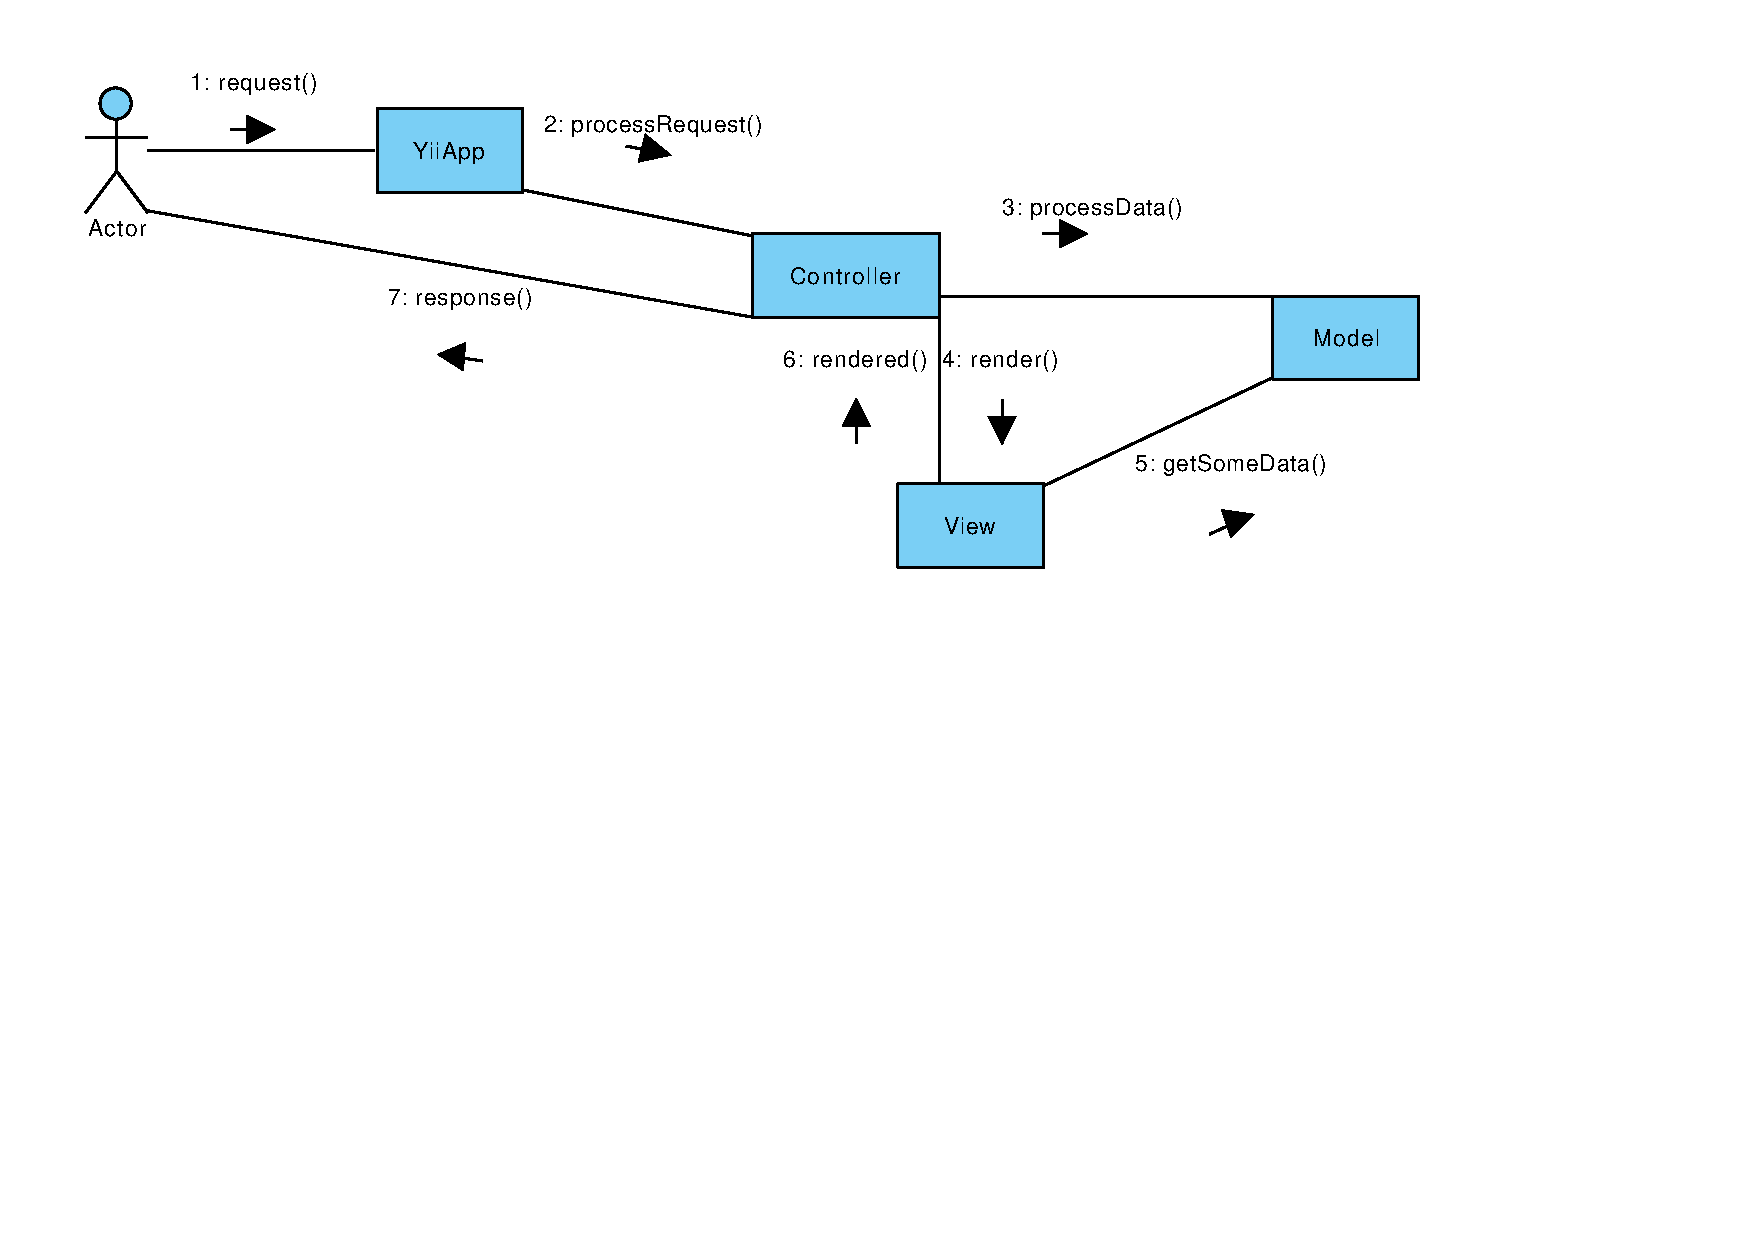
\includegraphics[scale=0.6, trim=0mm 100mm 40mm 0mm, clip]{../resources/uml/YiiRequestFlow.pdf}
\caption{Cхематичная диаграмма взаимодействия, демонстрирующая жизненный цикл пользовательского запроса в Yii}
\label{gr:yiirequestflow}
\end{center}
\end{figure} 

\paragraph{Архитектура фреймворка}
Все компоненты фреймворка разбиты на пакеты-слои, такие как: Контроллеры, Модели, Формы, 
Элементы представления. Причем для каждого слоя выделен отдельный базовый класс ---
 Layer Supertype\cite{fowler}. Кроме того определен базовый класс CComponent, от которого
унаследованы все супертипы слоев, в котором реализована работа с событиями.

Классы-формы используются как посредники между представлениями и моделями, пользователю
они доступны как обычная форма для ввода данных, после отправки которой обновленные данные
из запроса отображаются в поля объекта-модели.

При разработке приложения программисту доступен для использования глобальный объект-реестр,
с помощью которого можно получить доступ ко всем остальным глобальным объектам или сервисам.
Получение самого реестра реализована с применением типового решения Singleton\cite{gamma}.
Кроме всего прочего фреймворк предоставляет возможность разработчику самому добавлять в реестр
объекты-сервисы, которые должны быть доступны из любой точки приложения. 

\paragraph{Работа с БД}Встроенная ORM реализует паттерн проектирования Active Record\cite{fowler},
инкапсулируя работу с базой данных, при взаимодействии с объектами модели предметной области.

Кроме того для классов-моделей предлагаются удобные интерфейсы для определения правил проверки
корректности данных и задания названий полей с учетом мультиязычного интерфейса.

С помощью дополнительного расширения Giix\cite{giix} становится возможной генерация классов модели предметной
области на основе текущей структуры базы данных, причем:
\begin{enumerate}
\item{
  Для каждой таблицы(кроме используемых для реализации связи N:M) генерируется по два класса-модели:
  основной, который предназначен для дальнейшего изменения пользователем, и родительский класс 
  с префиксом ``Base'', в котором описывается логика отображения данных, и который может быть
  сгенерирован заново при изменении структуры таблицы. Также в базовом классе добавляются
  стандартные проверки корректности данных модели, такие как проверки, что формат значений полей объекта
  класса удовлетворяет формату типа соответствующего поля БД (например целое число или дата).
}
\item{
  На основе списка внешних ключей таблиц генерируются правила отображения связей объектов предметной области, 
  причем как для типа связей ``один-ко-многим'', так и для типа ``многие-ко-многим''.
  Таким образом после подгрузки из базы данных одного из объектов, через его поля можно осуществлять доступ
  к связанным с ним другим объектам классов модели предметной области.
}
\end{enumerate}

Кроме того Giix предоставляет механизмы для автоматической генерации, т.н. ``скаффолдинга'', кода с реализацией
CRUD-интерфейса для каждой из моделей. Полученный код чаще всего нуждается в дальнейшей настройке, однако 
служит удобной базой при разработке пользовательский интерфейсов для простых операций с объектами.

\paragraph{Консольные команды} При рассмотрении архитектуры Yii следует указать на возможность 
создания консольных команд в рамках фреймворка, реализация обработчиков которых сходна с 
реализацией контроллера страниц, за исключением того, что создаваемые классы должны быть унаследованы
от абстрактного класса ``CConsoleCommand''. 

Код команд может быть запущен из консоли в формате:

\textit{./yiic <CommandClassName> <ActionName> [args]*}

Данная возможность архитектуры Yii используется в частности при реализации фоновых задач (см. \ref{task:background}) 

\subsubsection{Запуск фоновых задач}
\label{task:background}
При проектировании системы можно выделить класс задач, каждая из которых
не может быть выполнена в рамках времени одного HTTP-запроса (средняя время обработки которого
не должно превышать одной секунды), но при этом их запуск должен быть инициирован через веб-интерфейс, и
пользователю по окончании выполнения задачи должны быть доступны резульаты работы. Такими задачами являются
импорт договоров по IPTV, расчет отчислений по Live, генерация статистических отчетов и т.д.

Для решения этой проблемы было принято решение воспользоваться стандартным для PHP инструментом 
``Gearman''\cite{gearman} --- которое по сути представляет собой фреймворк для распределения задач между множеством
машин для их параллельного исполнения. В рамках предоставляемого каркаса определены следующие типы объектов:
\begin{itemize}
\item{
  \textit{Задача} --- объект, содержащий наименование задачи (по сути название функции), аргументы и уникальный идентификатор.
}
\item{
  \textit{Очередь задач} --- актуальный список задач, ожидающих исполнения, хранящийся на сервере.
}
\item{
  \textit{Сервер} --- приложение, куда по специальному сетевому протоколу поступают новые задачи от клиентов.
}
\item{
  \textit{Клиент} --- приложение, инициирущее добавление новых задач на сервер.
}
\item{
  \textit{Worker} --- приложение, получающее по специальному сетевому протоколу задачи с сервера,
исполняющее задачи. После выполнения задачи результат выполнения может быть передан на сервер.
}
\end{itemize}

Стоит отметить, что может быть запущено несколько экземпляров приложения каждого типа, кроме того они могут находиться
на разных выделенных хостах. Единственное условие --- наличие доступа к серверу внутри сети для каждого из них.

\begin{figure}[!ht]
\begin{center}
\vspace{-0.5cm}
\hspace{20cm}
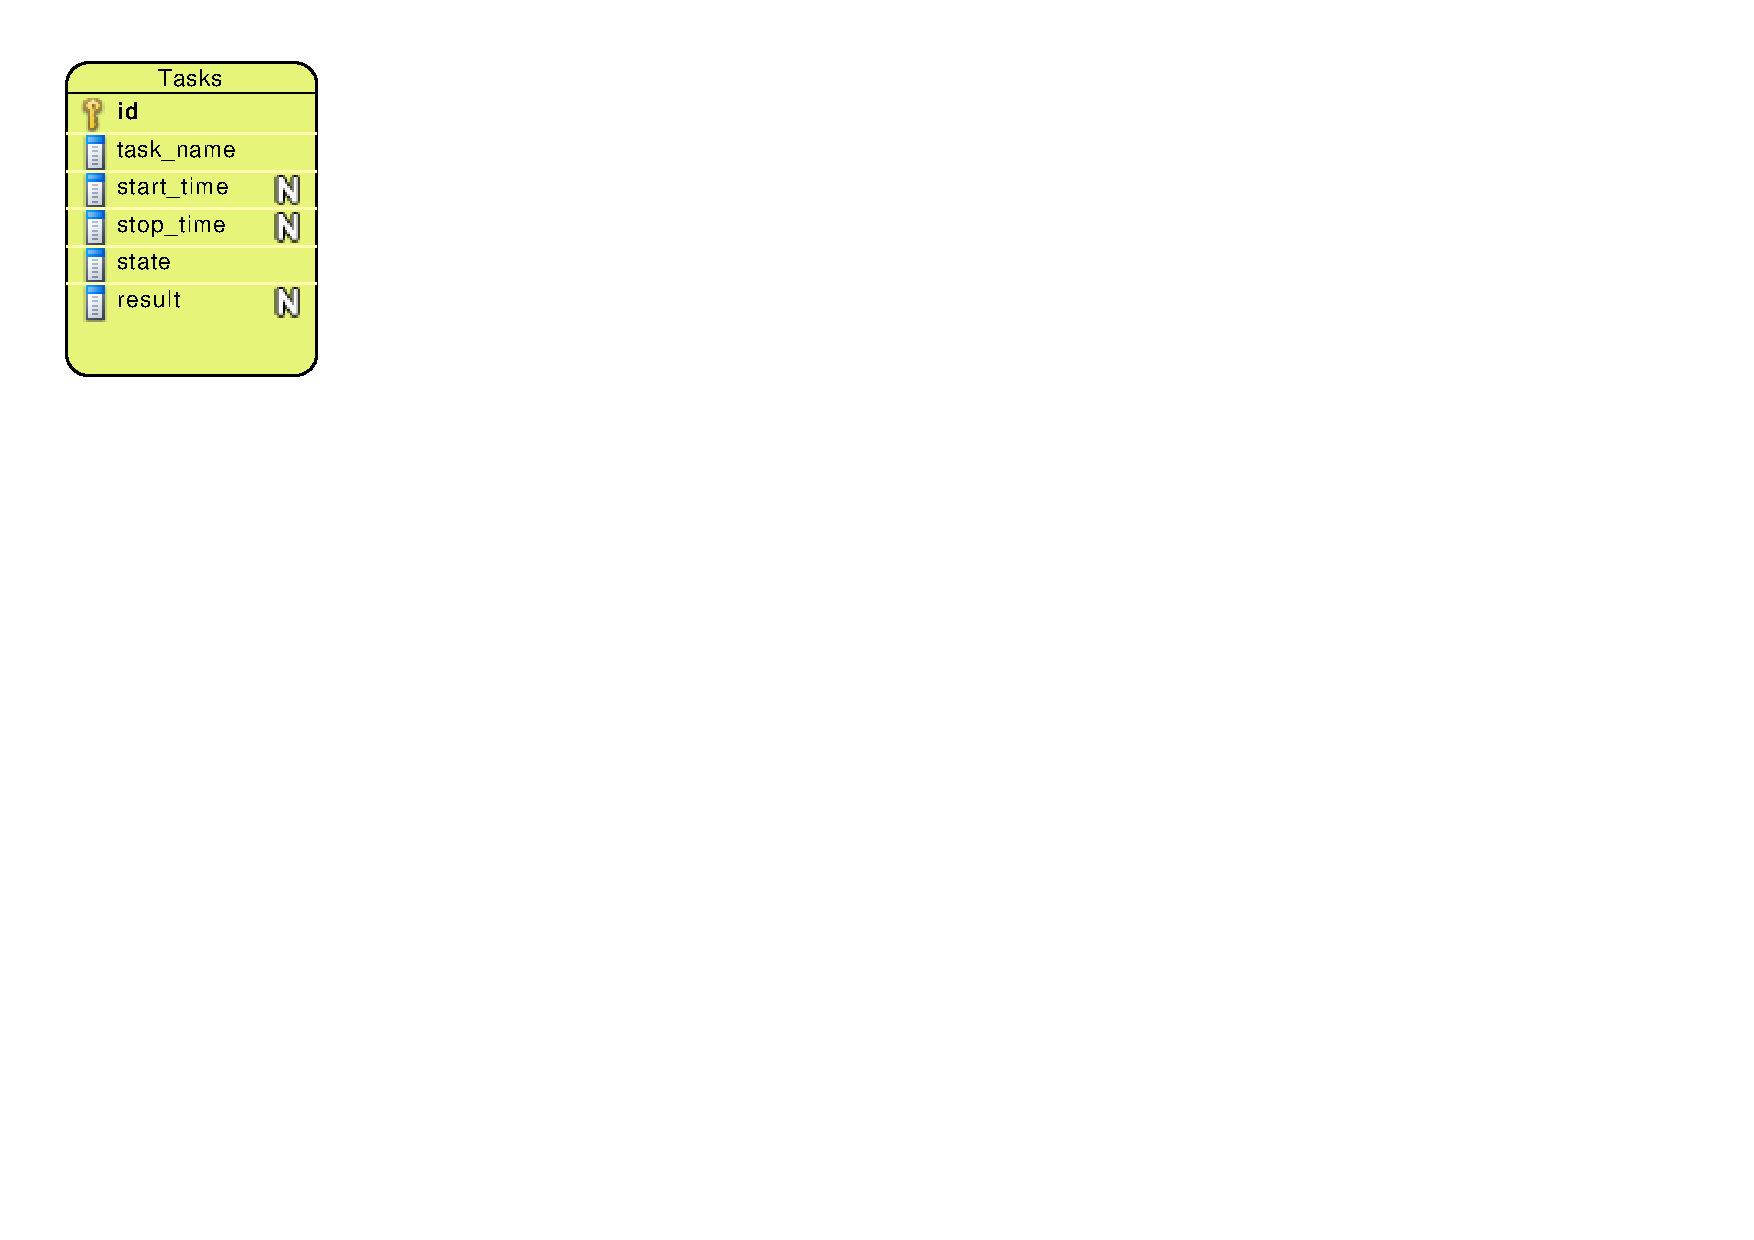
\includegraphics[scale=0.9, trim=10mm 143mm 240mm 10mm, clip]{../resources/uml/Tasks_db.pdf}
\caption{Диаграмма баркера для множества сущностей Tasks}
\label{gr:tasks_db}
\end{center}
\end{figure} 

В рамках разрабатываемой системы была принята к использованию следующая упрощенная архитектура использования
Gearman:
\begin{enumerate}
\item{
  Для каждого типа фоновых задач реализовать отдельный класс-контроллер консольного приложения, параметры 
  для задач должны приниматься в качестве аргументов команды.
}
\item{
  Приложения-воркеры реализуют очень простую функцию, которая просто запускает консольную команду,
   переданную в аругементах задачи (одно из приложений из п.1).
}
\item{
  При инициализации той или иной задачи пользователем, на сервер-супервизор отправляется новая задача,
  в качестве параметра передается консольная команда с аргументами, которая должна быть запущена.
}
\item{
  После отправки задачи на сервер в базе данных создается сущность Task с соответствующим идентификатором
  и именем (см. рис. \ref{gr:tasks_db}), а браузер пользователя перенаправляется на страницу
  ожидания результатов задачи, где при помощи ajax-запросов регулярно проверяется, была ли завершена задача.
  В момент завершения задачи, пользователю выводится уведомление. В случае построения отчета или в других
  случаях, когда результатом выполнения задачи служит файл, браузер пользователя инициирует его скачивание.
}
\item{
  В каждом из консольных предположений, использующихся для запуска фоновых задач, должна быть реализованы
  механизмы обновления статуса и сохранения результата в соотвествующей им сущности Task.
}
\end{enumerate}

Для упрощения создания новых реализаций команд, выполняющих фоновые задачи, был создан абстрактный класс
``AbstractTaskCommand'', унаследованный от ``CConsoleCommand'', переопределяющий некоторые из его методов
инкапсулируя работу с соответствующим объектом Task, обновляющий статус задачи в начале ее выполнения и после,
а так же отслеживающий возникновение исключений.
Таким образом при появлении новых задач, достаточно создать наследник класса AbstractTaskCommand с реализацией
логики самой задачи (см рис. \ref{gr:tasks_class}).

\begin{figure}[!ht]
\begin{center}
\vspace{-0.5cm}
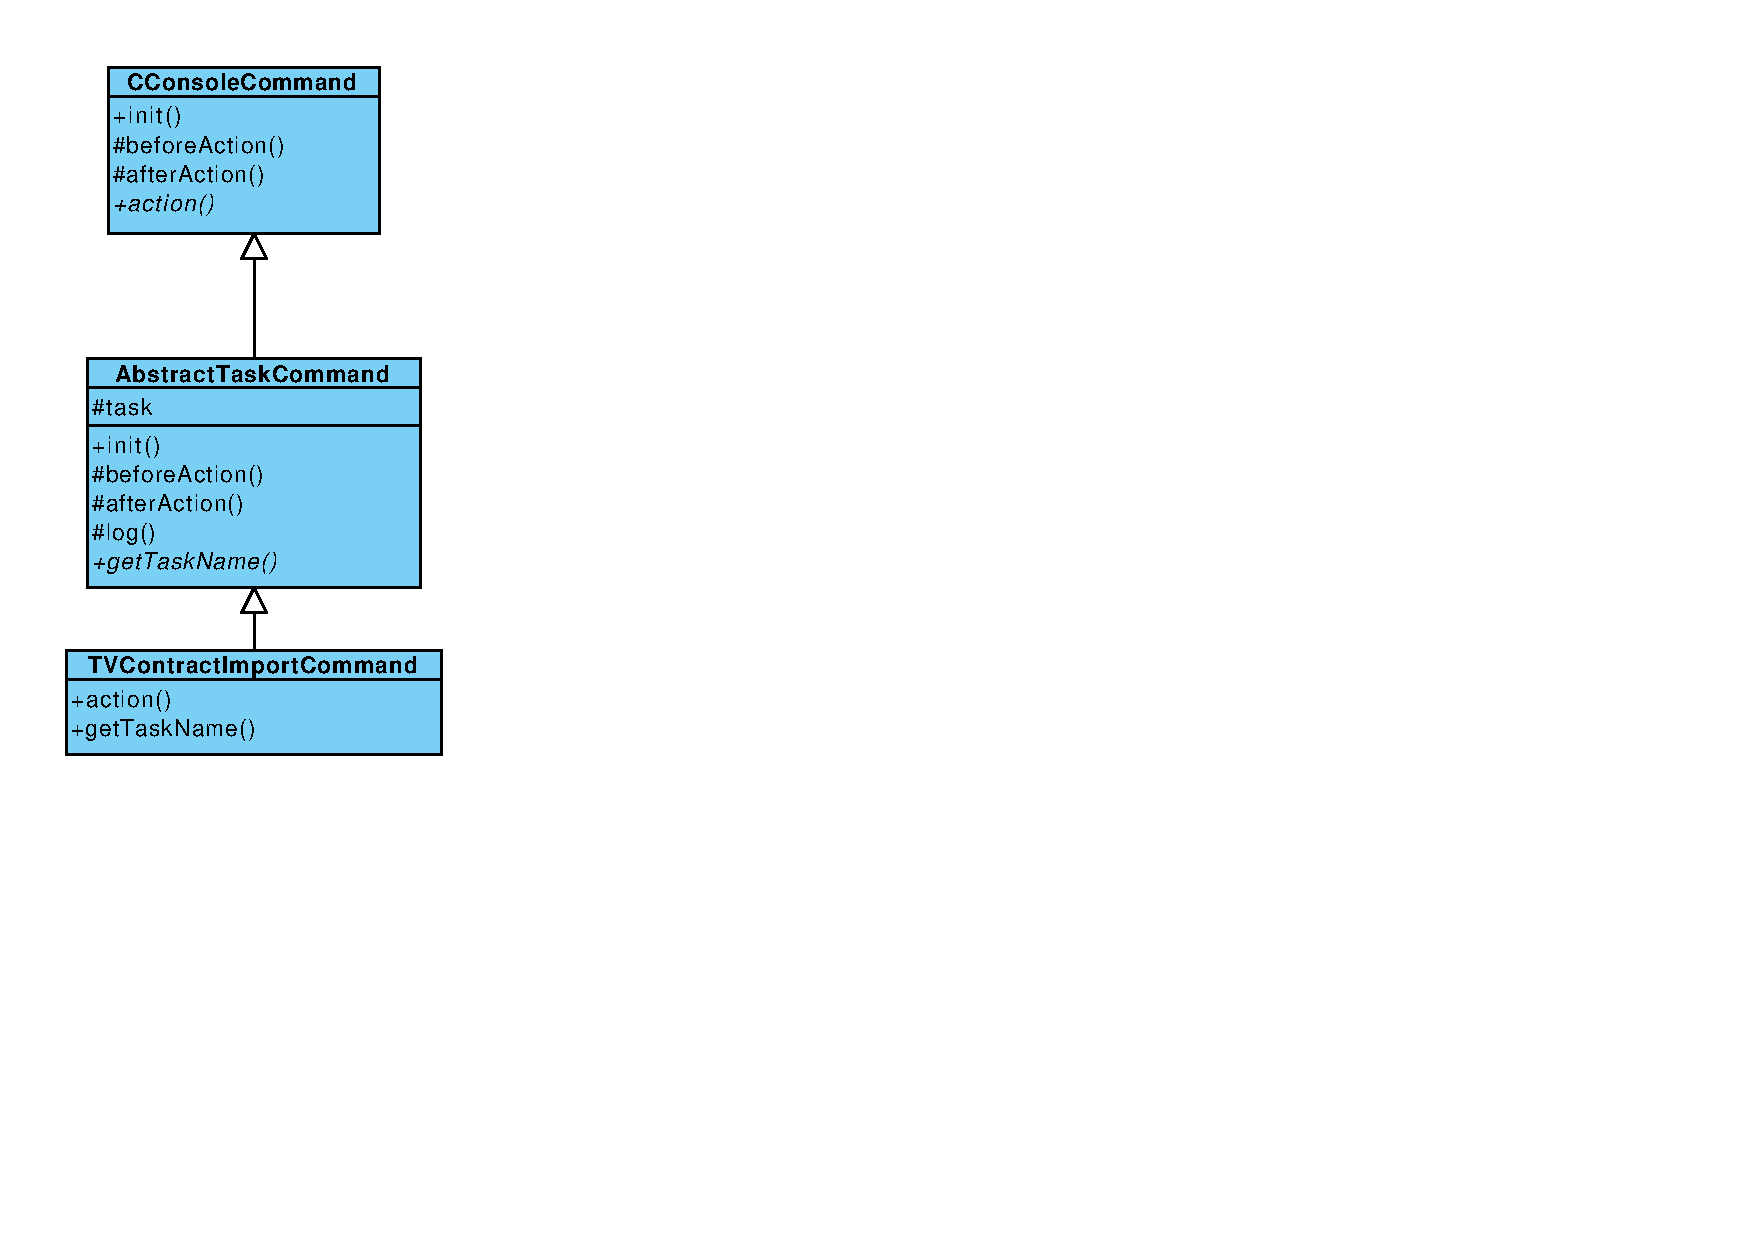
\includegraphics[scale=0.7, trim=10mm 81mm 200mm 10mm, clip]{../resources/uml/AbstractTask.pdf}
\caption{Диаграмма классов с примером реализации консольной команды ``Импорт договоров''}
\label{gr:tasks_class}
\end{center}
\end{figure} 

Описанное решение проблемы запуска фоновых задач делает такие трудоемкие операции, как построение отчетов
или расчет отчислений, в высокой степени горизонтально масштабируемыми за счет возможности увеличения
числа машин-воркеров.

\subsubsection{Диаграмма развертывания}
\begin{figure}[!ht]
\begin{center}
\vspace{-0.5cm}
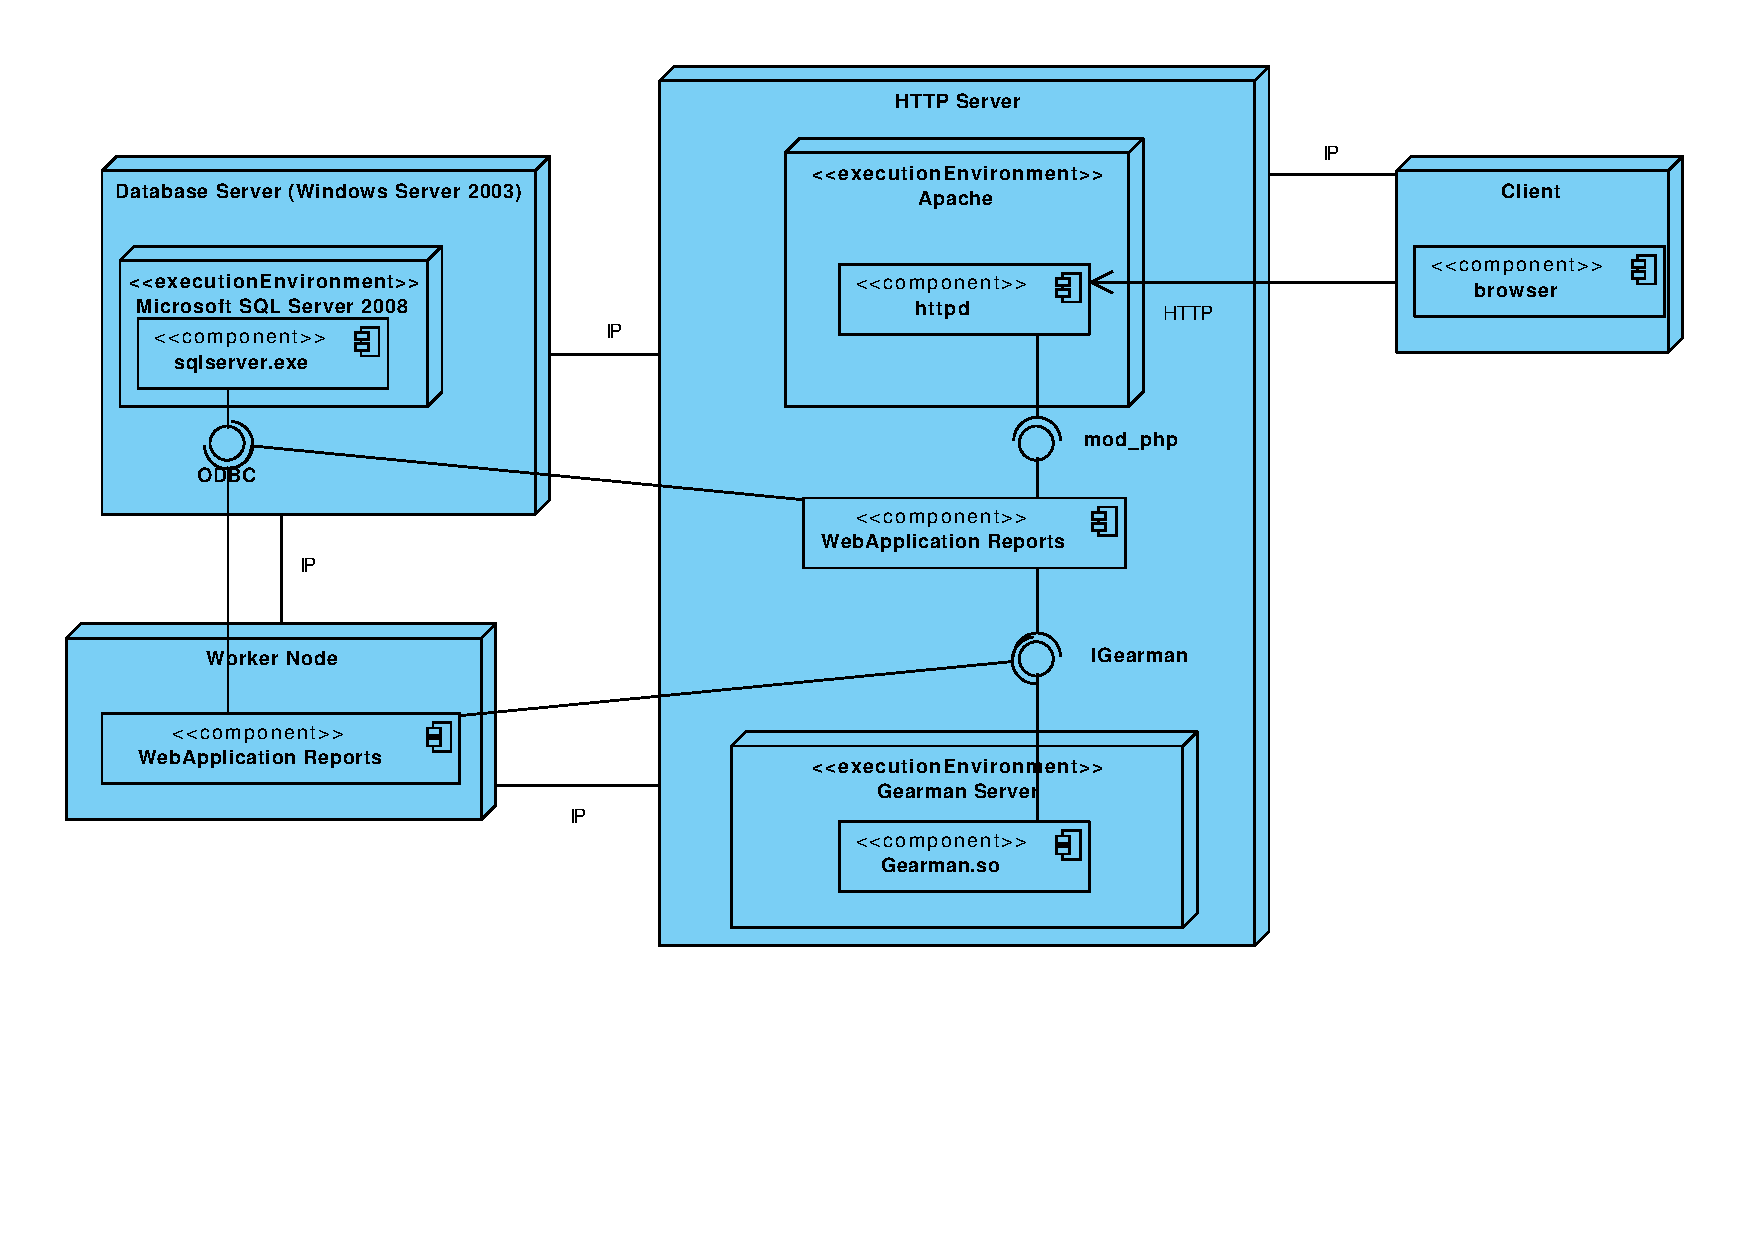
\includegraphics[scale=0.6, trim=10mm 50mm 0mm 10mm, clip]{../resources/uml/Deployment.pdf}
\caption{Схематичная диаграмма развертывания системы}
\label{gr:deployment}
\end{center}
\end{figure} 

Из диаграммы развертывания системы (рис. \ref{gr:deployment}) видно, что в качестве веб-сервера
системы предлагается к использованию Apache, который соединен с приложением с помощью модуля \textit{mod\_php}.
Веб-приложение Reports соединяется с СУБД Microsoft SQL Server 2008, находящейся на выделенном
сервере под управлением операционной системы Windows Server 2003, посредством протокола ODBC.
Сервер очередей задач Gearman располагается на том же хосте, что и веб-приложение, а экземпляры-воркеры
могут быть запущены на отдельном сервере, имеющем сетевой доступ, как к основному серверу,
так и к серверу СУБД.

\subsection{Структура базы данных}
В этом разделе описана структура базы данных, разработанная для системы LM Reports.
Предлагается описание структуры в виде диаграмм Баркера, каждая из которых в достаточной степени
подробно описывает отдельные участки модели предметной области. 

Множества сущностей в диаграммах названы на русском языке для удобства читателя при сопоставлении
элементов бизнес-логики, описанных в первой главе, и объектов диаграммы.
В диаграммах отмечены поля, образующие первичные, потенциальные и внешние ключи множеств сущностей. 
Почти для всех множеств введен суррогатный первичный ключ.

\newpage
\subsubsection{Отчисления Live}

\begin{figure}[!ht]
\begin{center}
\vspace{-0.5cm}
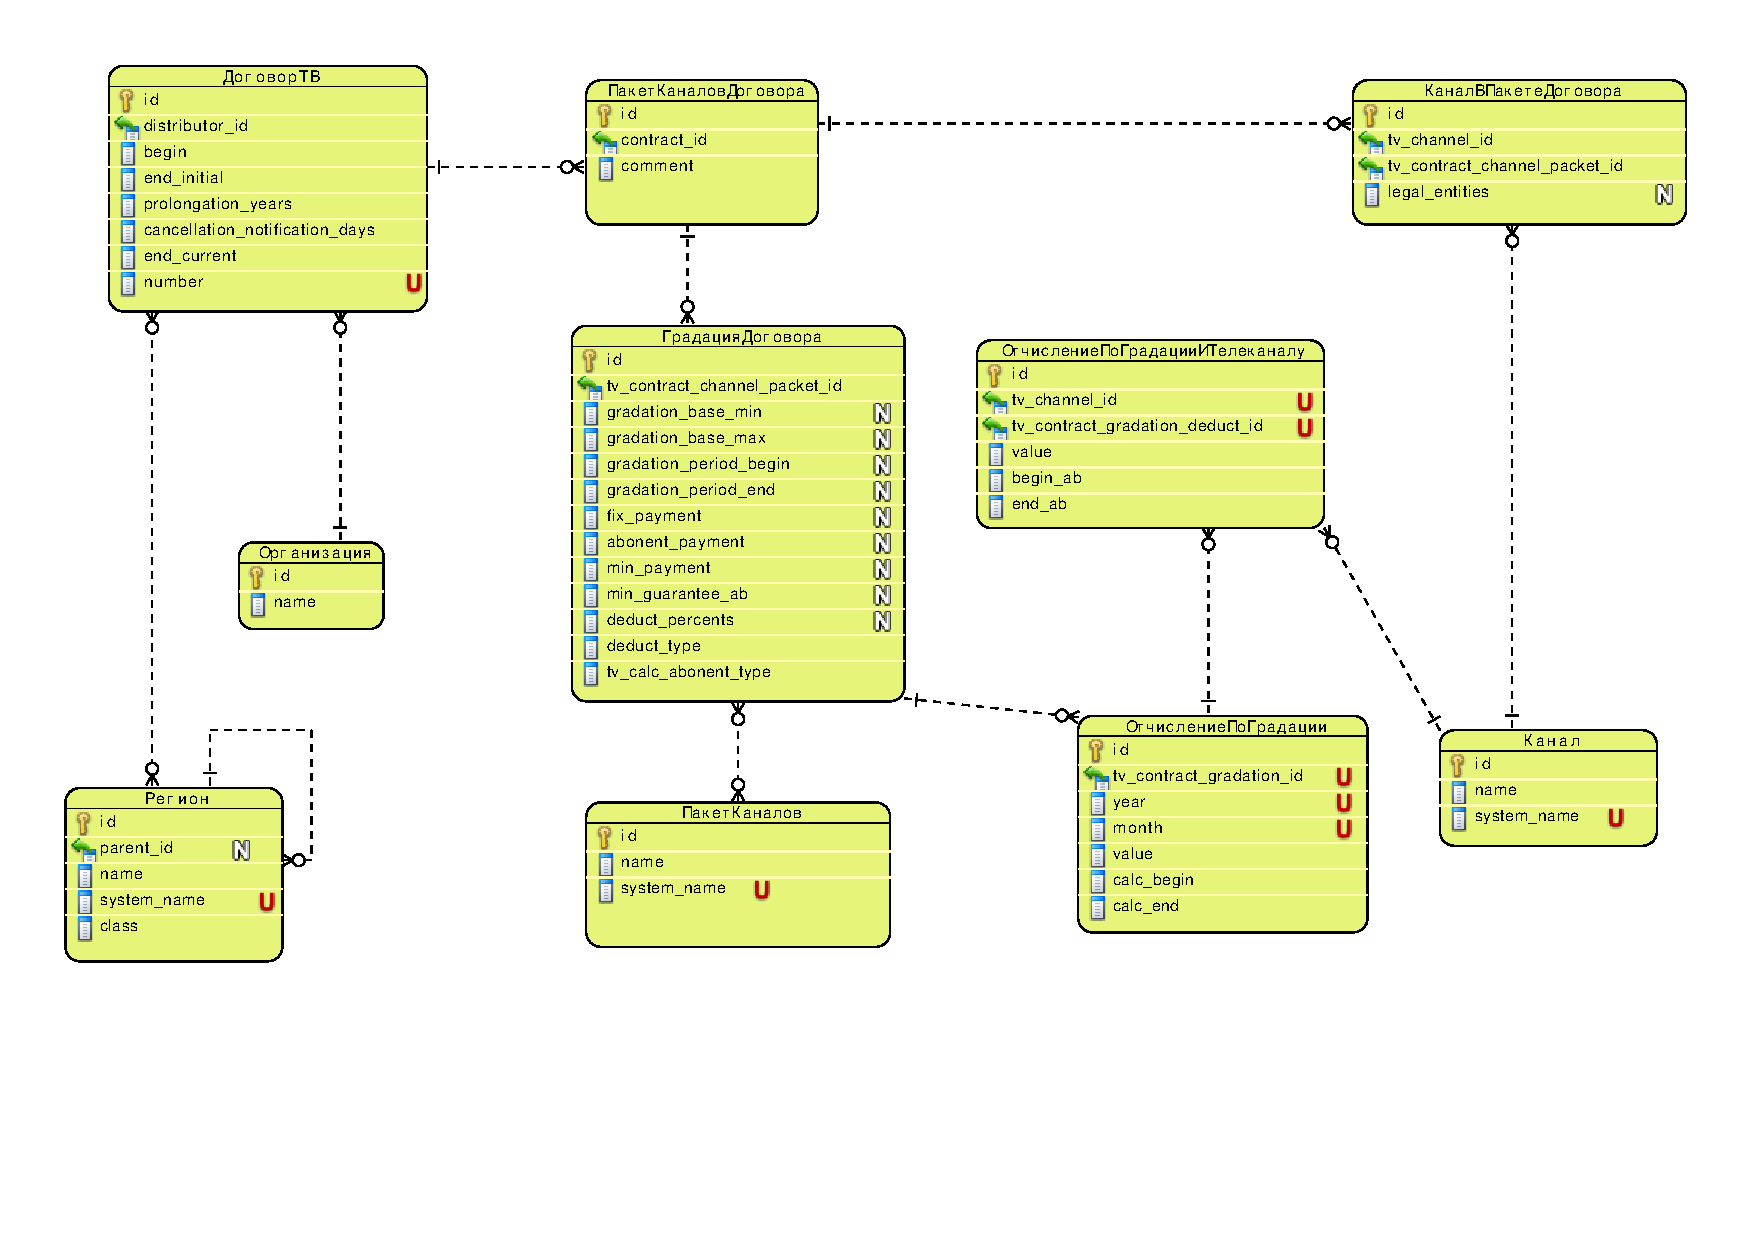
\includegraphics[scale=0.65, trim=10mm 40mm 0mm 10mm, clip]{../resources/uml/TV_DEDUCT.pdf}
\caption{Диаграмма Баркера, демонстрирующая структуру БД для отчислений по Live}
\label{gr:tv_deduct}
\end{center} 
\end{figure}


\paragraph{Справочники} В диаграмме (рис. \ref{gr:tv_deduct}) затронуто описание некоторых справочных
множеств сущностей:
\begin{itemize}
\item{
  \textit{Организация} --- с двумя атрибутами --- идентификатором и названием.
}
\item{
  \textit{Регион} содержит наименование, системное название (в биллинге провайдера), класс территории (тип ENUM),
  и ссылку на родительский регион.
}
\item{
  \textit{Пакет каналов} и \textit{Канал} содержат названия, системные наименования (уникальные идентификаторы).
}
\end{itemize} 

\paragraph{Договоры по Live} В множестве сущностей \textit{ДоговорТВ} отображены договоры по Live, их поля:
\begin{itemize}
\item{
  \textit{distributor\_id} --- внешний ключ, ссылающийся на организацию-правообладатель
}
\item{
  \textit{Номер договора} уникальный номер договора со сквозной нумерацией.
}
\item{
  \textit{Начало действия договора}, \textit{Окончание действия договора (изначальное)}, \textit{Продление срока действия договора (в годах)}
 описывают временной интервал, в котором данный договор является действующим.
}
\end{itemize}

\paragraph{Градации договора} В множестве сущностей \textit{ГрадацияДоговора} отображены градации договоров по Live (см. \ref{live:deducts}), их поля:
\begin{itemize}
\item{
  \textit{gradation\_base\_min, gradation\_base\_max, gradation\_period\_begin, gradation\_period\_end}  
    --- описывают условия применимости градации по базе и по сроку.
}
\item{
  \textit{deduct\_type} и \textit{tv\_calc\_abonent\_type} --- схема расчета и вид расчета базы абонентов градации (тип ENUM).
}
\item{
  \textit{fix\_payment}, \textit{abonent\_payment}, \textit{min\_payment}, \textit{min\_guarantee\_ab},
  \textit{deduct\_percent} --- соответственно ``фиксированный платеж'', ``платеж за абонента'', ``мин.платеж'',
  ``минимальное гарантированное число абонентов'', ``процент отчислений''.
}
\end{itemize}
Следует учитывать, что некоторые из этих полей могут быть незаполненными, что отмечено в диаграмме стереотипом ``N''.

\paragraph{Отчисления по градации} Множество сущностей \textit{ОтчислениеПоГрадации}, которое заполняется 
при расчете отчислений по Live. Сущности, как следует из названия, принадлежат ровно одной градации, соотвественно определен
внешний ключ \textit{tv\_contract\_gradation\_id}.
\begin{itemize}
\item{
  \textit{year} и \textit{month} --- год и номер месяца, для которых был произведен расчет отчислений. 
  Вместе с \textit{tv\_contract\_gradation\_id} составляют потенциальный ключ.
}
\item{
  \textit{calc\_begin} и \textit{calc\_end} --- начало и окончание периода, для которого был произведен расчет отчислений.
  В общем случае могут не соответствовать границе месяца, так как необязательно градация применима для всего месяца.
}
\item{
  \textit{value} --- величина конкретного отчисления (значение в рублях с точностью до $10^{-3}$). 
}
\end{itemize}

\paragraph{Разбивка отчисления} Множество сущностей \textit{ОтчислениеПоГрадацииИТелеканалу}, опреляет величину отчислений
для каждого телеканала пакета градации. 
Каждый объект принадлежит одному из отчислений по градации, а также телеканалу, причем внешние ключи
\textit{tv\_contract\_gradation\_deduct\_id} и \textit{tv\_channel\_id} формируют потенциальный ключ отношения.
\begin{itemize}
\item{
  \textit{begin\_ab} и \textit{end\_ab} --- количество абонентов телеканала на начало и конец периода расчета, 
на основе которого происходил расчет.
}
\item{
  \textit{value} --- величина конкретного отчисления (значение в рублях с точностью до $10^{-3}$). 
}
\end{itemize}

\subsubsection{Статистические данные Live}
\begin{figure}[!ht]
\begin{center}
\vspace{-0.5cm}
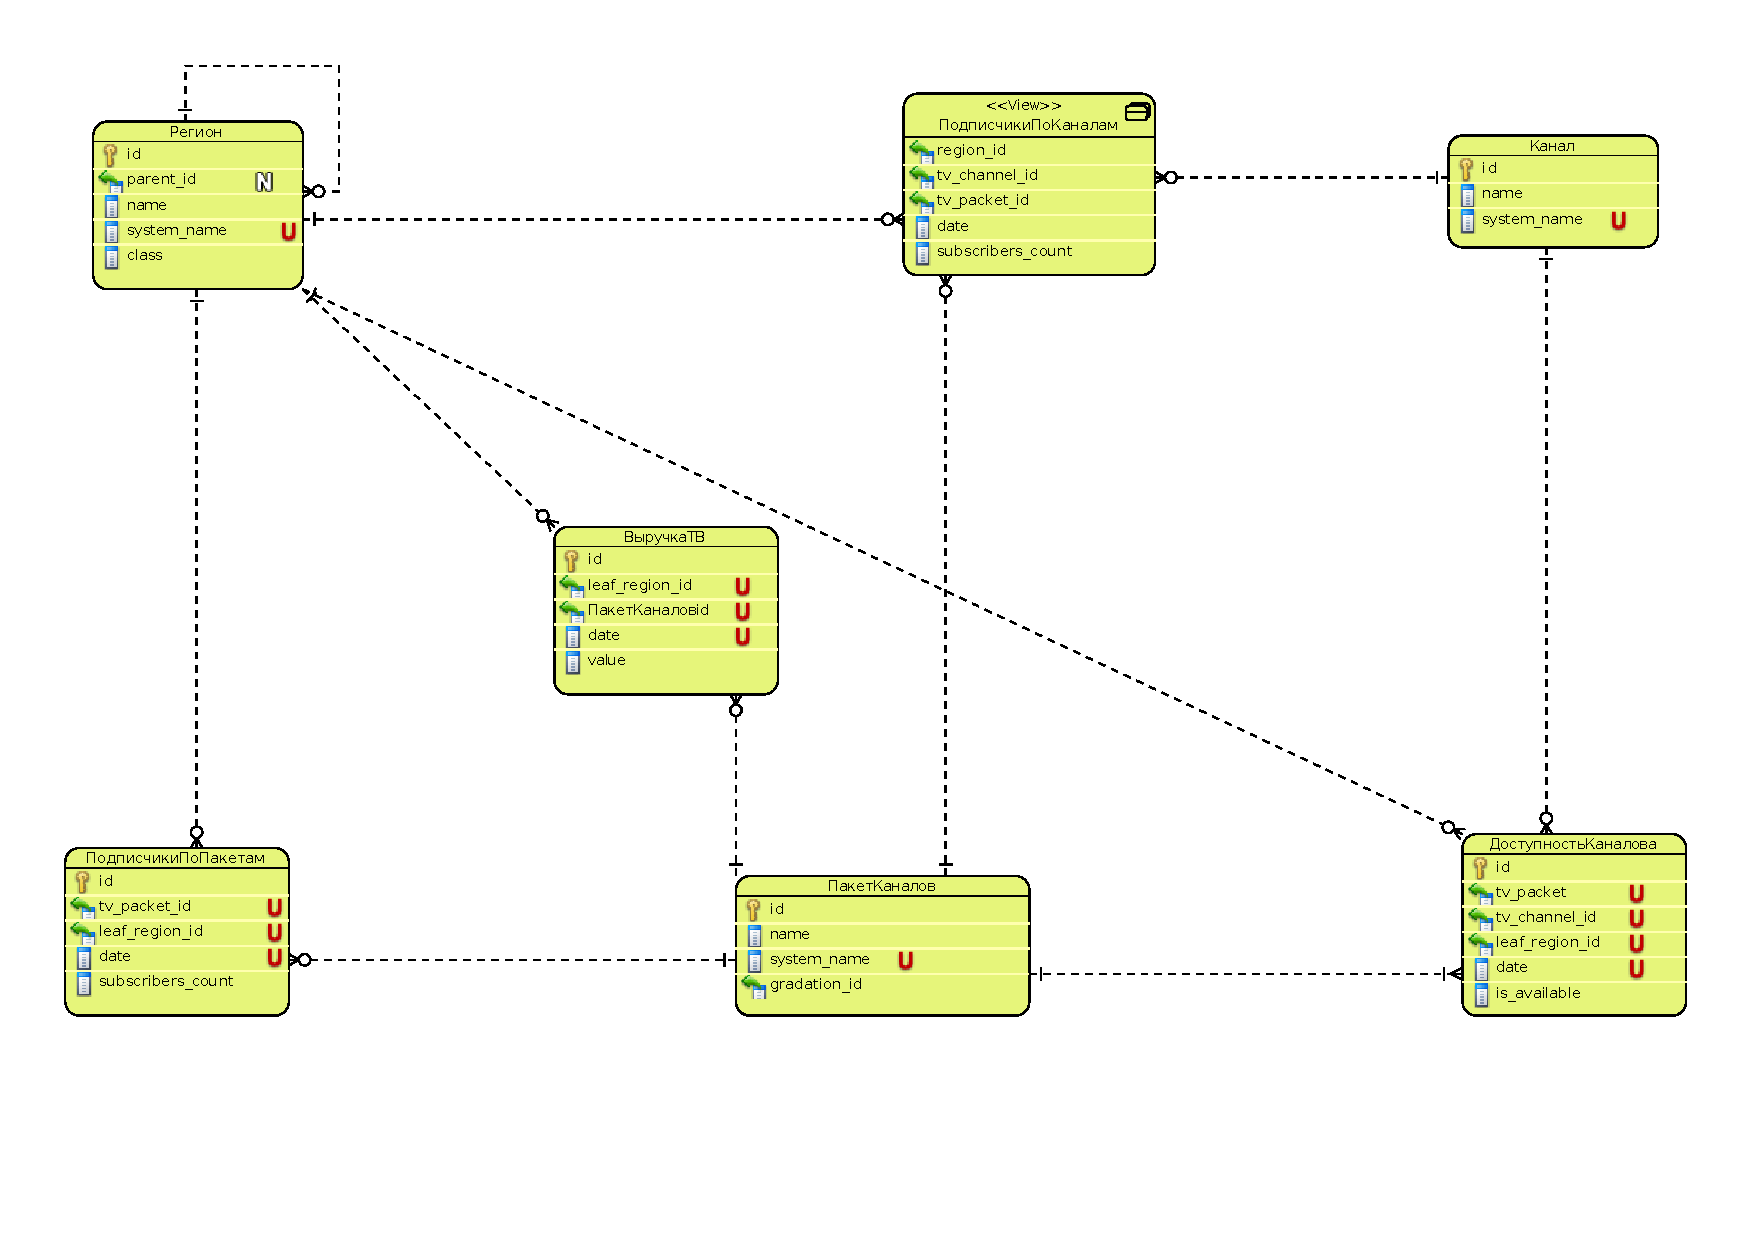
\includegraphics[scale=0.65, trim=10mm 30mm 0mm 10mm, clip]{../resources/uml/TV_STAT.pdf}
\caption{Диаграмма Баркера, демонстрирующая структуру БД для статистических данных по Live}
\label{gr:tv_deduct}
\end{center} 
\end{figure}

\paragraph{Абонентская база} Множество сущностей \textit{ПодписчикиПоПакетам} определяет размер
абонентской базы для каждого из пакетов телеканалов в территориях-листьях на каждый день (см. \ref{stat:live}).
\begin{itemize}
\item{
  \textit{tv\_packet\_id} и \textit{leaf\_region\_id} --- внешние ключи для множеств сущностей ``Пакет телеканалов`` и
  ``Регион''.
}
\item{
  \textit{date} --- дата, для которой указано число подсписчков. Вместе со ссылками на пакет и территорию
образует потенциальный ключ.
}
\item{
  \textit{subscribers\_count} --- число подписчиков. 
}
\end{itemize}

\paragraph{Доступность каналов} определяет какие телеканалы были доступны в пакете в определенную дату в пакете для территории.
\begin{itemize}
\item{
  \textit{tv\_packet\_id}, \textit{leaf\_region\_id} и \textit{tv\_channel\_id} --- внешние ключи для множеств сущностей 
``Пакет телеканалов``, ``Регион'' и ``Канал''.
}
\item{
  \textit{date} --- дата, для которой указано число подсписчков. Вместе со ссылками на пакет, территорию и телеканал
образует потенциальный ключ.
}
\item{
  \textit{is\_available} --- параметр доступности, возможные значения --- 0/1. 
}
\end{itemize}

\paragraph{ВыручкаТВ} определяет размер выручки, полученной провайдером для каждого из пакетов телеканалов в территориях-листьях 
за каждый день. Структура аналогична множеству ``ПодписчикиПоПакетам'' за исключением того, что вместо атрибута 
\textit{subscribers\_count} в множестве определен \textit{value}, в котором хранится сумма выручки в рублях с точностью до $10^{-2}$.

\paragraph{ПодписчикиПоКаналам} виртуальное множество сущностей (View), построенное на основе двух других:
``ПодписчикиПоПакетам`` и ``ДоступностьКаналов'', определяющая усредненное число подписчиков по телеканалу в регионе
за определенную дату.

